\documentclass[conference]{IEEEtran}

\usepackage{cite}
\usepackage{amsmath,amssymb}
\usepackage{graphicx}
\usepackage{array}
\usepackage{booktabs}
\usepackage{xcolor}
\usepackage{url}

\begin{document}

\title{AgriDirect: A Smart Farm-to-Customer Marketplace with Weather-Aware Crop Advisory and Market Intelligence}

\author{
\IEEEauthorblockN{M.Hemasai}
\IEEEauthorblockA{
Department of ACSE \\
Vignan's Foundation for Science, Technology and Research \\
Guntur, Andhra Pradesh, India \\
231fa18039@gmail.com
}
\and
\IEEEauthorblockN{K.Sreelatha}
\IEEEauthorblockA{
Department of ACSE \\
Vignan's Foundation for Science, Technology and Research \\
Guntur, Andhra Pradesh, India \\
231fa18051@gmail.com
}
\and
\IEEEauthorblockN{G.Udaya}
\IEEEauthorblockA{
Department of ACSE \\
Vignan's Foundation for Science, Technology and Research \\
Guntur, Andhra Pradesh, India \\
231fa18075@gmail.com
}
\and
\IEEEauthorblockN{M.Eswar}
\IEEEauthorblockA{
Department of ACSE \\
Vignan's Foundation for Science, Technology and Research \\
Guntur, Andhra Pradesh, India \\
231fa18422@gmail.com
}
\and
\IEEEauthorblockN{Arnab De}
\IEEEauthorblockA{
Department of ACSE \\
Vignan's Foundation for Science, Technology and Research \\
Guntur, Andhra Pradesh, India \\
ade.ece1990@gmail.com
}
}

\maketitle

\begin{abstract}
Agricultural commerce often suffers from fragmented supply chains, weak price transparency, and limited decision support for farmers. This paper presents AgriDirect, a full-stack digital platform designed to connect farmers and customers through direct produce trading while also assisting cultivation decisions with weather-aware crop advisory and live mandi price intelligence. The system combines a React-based client application, an Express and MongoDB backend, and a FastAPI-based machine learning service for crop recommendation. Farmers can manage inventory, monitor market trends, review weather conditions, and obtain ranked crop suggestions using farm inputs and market context. Customers can discover grouped products, compare sellers, select nearby sources, and place secure orders. The proposed platform demonstrates how e-commerce workflows, geolocation, public market data, and intelligent advisory components can be unified in a single agriculture-focused application. AgriDirect aims to improve transparency, reduce dependency on intermediaries, and support better operational decisions for both producers and consumers.
\end{abstract}

\begin{IEEEkeywords}
smart agriculture, e-commerce, crop recommendation, mandi price analytics, weather forecasting, full-stack application
\end{IEEEkeywords}

\section{Introduction}
Agriculture remains a major economic activity, yet many farmers still face difficulty in receiving fair prices and timely market information. Traditional supply chains often involve multiple intermediaries, which can reduce farmer margins and limit transparency for end customers. At the same time, crop planning decisions are increasingly affected by local climate variation, market volatility, and access to digital services.

To address these issues, AgriDirect is designed as a farm-to-customer digital marketplace with integrated decision-support features. Instead of functioning only as an online store, the platform combines agricultural commerce with advisory intelligence. Farmers can list produce, track stock levels, observe mandi prices, and obtain crop suggestions using environmental conditions and farm profile inputs. Customers can browse products, compare sellers, and place orders directly through the same ecosystem.

The main contribution of this work is the design and implementation of a unified agriculture platform that merges marketplace operations with practical advisory services. The project focuses on three goals: direct digital trade, operational transparency, and intelligent support for crop planning.

\section{Literature Survey}
Digital agriculture platforms and smart marketplace systems have gained attention because they can reduce supply chain inefficiencies and improve farmer access to market information. Earlier agricultural commerce systems mainly focused on online buying and selling, inventory visibility, and digital order handling. While such systems improved accessibility, most of them did not integrate advisory intelligence for crop planning or environmental awareness.

Recent studies in smart farming have shown that machine learning and data-driven decision support can improve agricultural planning. Crop recommendation systems commonly use soil properties, rainfall, temperature, and humidity as predictive inputs. Techniques such as Random Forest, decision-tree-based learning, and rule-based inference are frequently used because they perform well on structured agricultural data. However, many existing recommendation tools operate as standalone utilities and are not connected to real marketplace outcomes.

Another important research direction involves agricultural price intelligence. Public mandi datasets and market feeds help estimate prevailing rates across regions, allowing farmers to better understand price trends and selling opportunities. Yet, most existing applications either visualize market data separately or use it only for reporting purposes rather than combining it directly with crop recommendation and product listing workflows.

From the e-commerce side, location-aware marketplaces have become increasingly important for perishable goods. Systems that compare seller distance, stock, and price can improve buyer convenience and freshness assurance. Even so, these systems often lack farmer-side strategic tools such as weather-driven crop suggestion, seasonal guidance, or market-sensitive ranking.

Based on this gap, AgriDirect is positioned as an integrated platform that combines direct produce trading, location-aware seller discovery, weather summarization, mandi intelligence, and crop advisory support in one architecture.

\section{Proposed System}
The proposed system, AgriDirect, is a smart agriculture marketplace designed to unify trading and advisory workflows. Instead of treating product selling, weather information, market rates, and crop guidance as separate modules, the platform links them into a single decision-support environment for farmers and customers.

The system allows farmers to list produce, monitor stock, analyze mandi trends, save advisory profiles, and request ranked crop suggestions. Customers can browse grouped produce, compare multiple sellers, identify nearby sources, add items to cart, and place orders through online or offline payment methods. The system also supports role-based access for farmers, customers, and administrators.

AgriDirect follows a multi-service architecture composed of a frontend client, an application backend, a database layer, and an auxiliary machine learning service. The frontend is developed using React and Vite, while the backend is built with Express.js and MongoDB. A separate FastAPI microservice is used to serve crop recommendation predictions.

\begin{figure}[htbp]
\centering
\fbox{
\begin{minipage}{0.47\textwidth}
\centering
\textbf{AgriDirect Architecture} \\[4pt]
Customers/Farmers $\rightarrow$ React Frontend \\[2pt]
React Frontend $\rightarrow$ Express API Layer \\[2pt]
Express API Layer $\rightarrow$ MongoDB \\[2pt]
Express API Layer $\rightarrow$ Weather API \\[2pt]
Express API Layer $\rightarrow$ Mandi Price API \\[2pt]
Express API Layer $\leftrightarrow$ FastAPI Crop Advisory Service
\end{minipage}
}
\caption{High-level architecture of the AgriDirect platform.}
\label{fig:architecture}
\end{figure}

The architecture separates user interaction, business logic, data persistence, and recommendation services. This separation improves maintainability and makes the platform extensible for future smart agriculture modules.

\section{System Implementation}
\subsection{Frontend Layer}
The frontend provides separate experiences for farmers, customers, and administrators. Protected routes are used to control role-based access. Farmers interact with product management, weather updates, mandi dashboards, and crop advisory views. Customers interact with product browsing, seller comparison, cart handling, profile management, and order placement.

\subsection{Backend Layer}
The Express backend exposes REST APIs for authentication, product management, customer operations, orders, mandi data retrieval, and advisory profile storage. MongoDB is used to persist users, products, and orders. The backend also computes seller distance using stored latitude and longitude values, enabling location-aware discovery.

\subsection{Crop Advisory Layer}
The crop advisory pipeline combines rule-based scoring with machine learning assistance. In the implemented system, farm inputs such as soil type, soil pH, irrigation level, season, average temperature, average humidity, and recent rainfall are used to rank candidate crops. In addition, mandi price information is used to introduce market-aware weighting to the recommendation score.

For a crop $c$, the final score can be interpreted as
\begin{equation}
S(c) = S_{\text{farm}}(c) + S_{\text{market}}(c)
\end{equation}
where $S_{\text{farm}}(c)$ captures agronomic suitability and $S_{\text{market}}(c)$ captures mandi-price-based opportunity. The score is then normalized to produce a ranked recommendation list.

\subsection{Machine Learning Service}
The auxiliary FastAPI service uses a trained crop model to generate top crop predictions from weather and soil-related inputs. The current implementation loads serialized model artifacts and label encoders, accepts environmental parameters through a prediction endpoint, and returns the top recommendations with confidence values.

\subsection{Data Flow and Processing Pipeline}
The end-to-end workflow of AgriDirect begins when a farmer or customer interacts with the frontend interface. Authentication data, product information, order requests, and advisory inputs are routed to the Express backend, which validates requests and communicates with the MongoDB database. For advisory tasks, the backend combines stored user profile data with weather summaries and mandi-price information before generating a ranked output. This flow ensures that the recommendation logic is not isolated from the operational state of the platform.

For farmers, the data flow is especially important because the advisory output depends on multiple layers: saved advisory profile, selected season, weather observations, and market conditions. For customers, the flow includes grouped product retrieval, seller lookup, and distance-aware comparison based on stored location information. This integrated request cycle makes AgriDirect closer to a decision-support system than a conventional listing application.

\subsection{Functional Modules}
The platform supports user registration, login, password management, and role-aware access for farmer, customer, and admin accounts. Farmers can add products, update price and quantity, remove inactive listings, and track stock levels. Each active listing is associated with a master product entry to maintain category consistency across the platform. Customers can browse grouped products, inspect available sellers for a selected item, compare price and distance, and add items to a cart before placing an order. The system also supports order creation, order history, payment-state tracking, and online payment integration through Razorpay.

\subsection{Technology Stack}
Table~\ref{tab:stack} summarizes the main technologies used in the project.

\begin{table}[htbp]
\caption{Technology Stack Used in AgriDirect}
\label{tab:stack}
\centering
\begin{tabular}{>{\raggedright\arraybackslash}p{0.22\linewidth} >{\raggedright\arraybackslash}p{0.22\linewidth}}
\toprule
\textbf{Component} & \textbf{Technology} \\
\midrule
Frontend & React, Vite, Tailwind CSS \\
Backend & Node.js, Express.js \\
Database & MongoDB, Mongoose \\
ML Service & FastAPI, scikit-learn \\
Mapping/Location & Latitude--longitude based distance logic \\
Charts/UI & Recharts, React Router \\
Payments & Razorpay \\
External Data & Weather API, mandi price API \\
\bottomrule
\end{tabular}
\end{table}

The modular structure of the implementation enables separation of concerns across client pages, API routes, controller logic, models, and advisory services. This organization supports future extension without major structural redesign.

\begin{figure}[htbp]
\centering
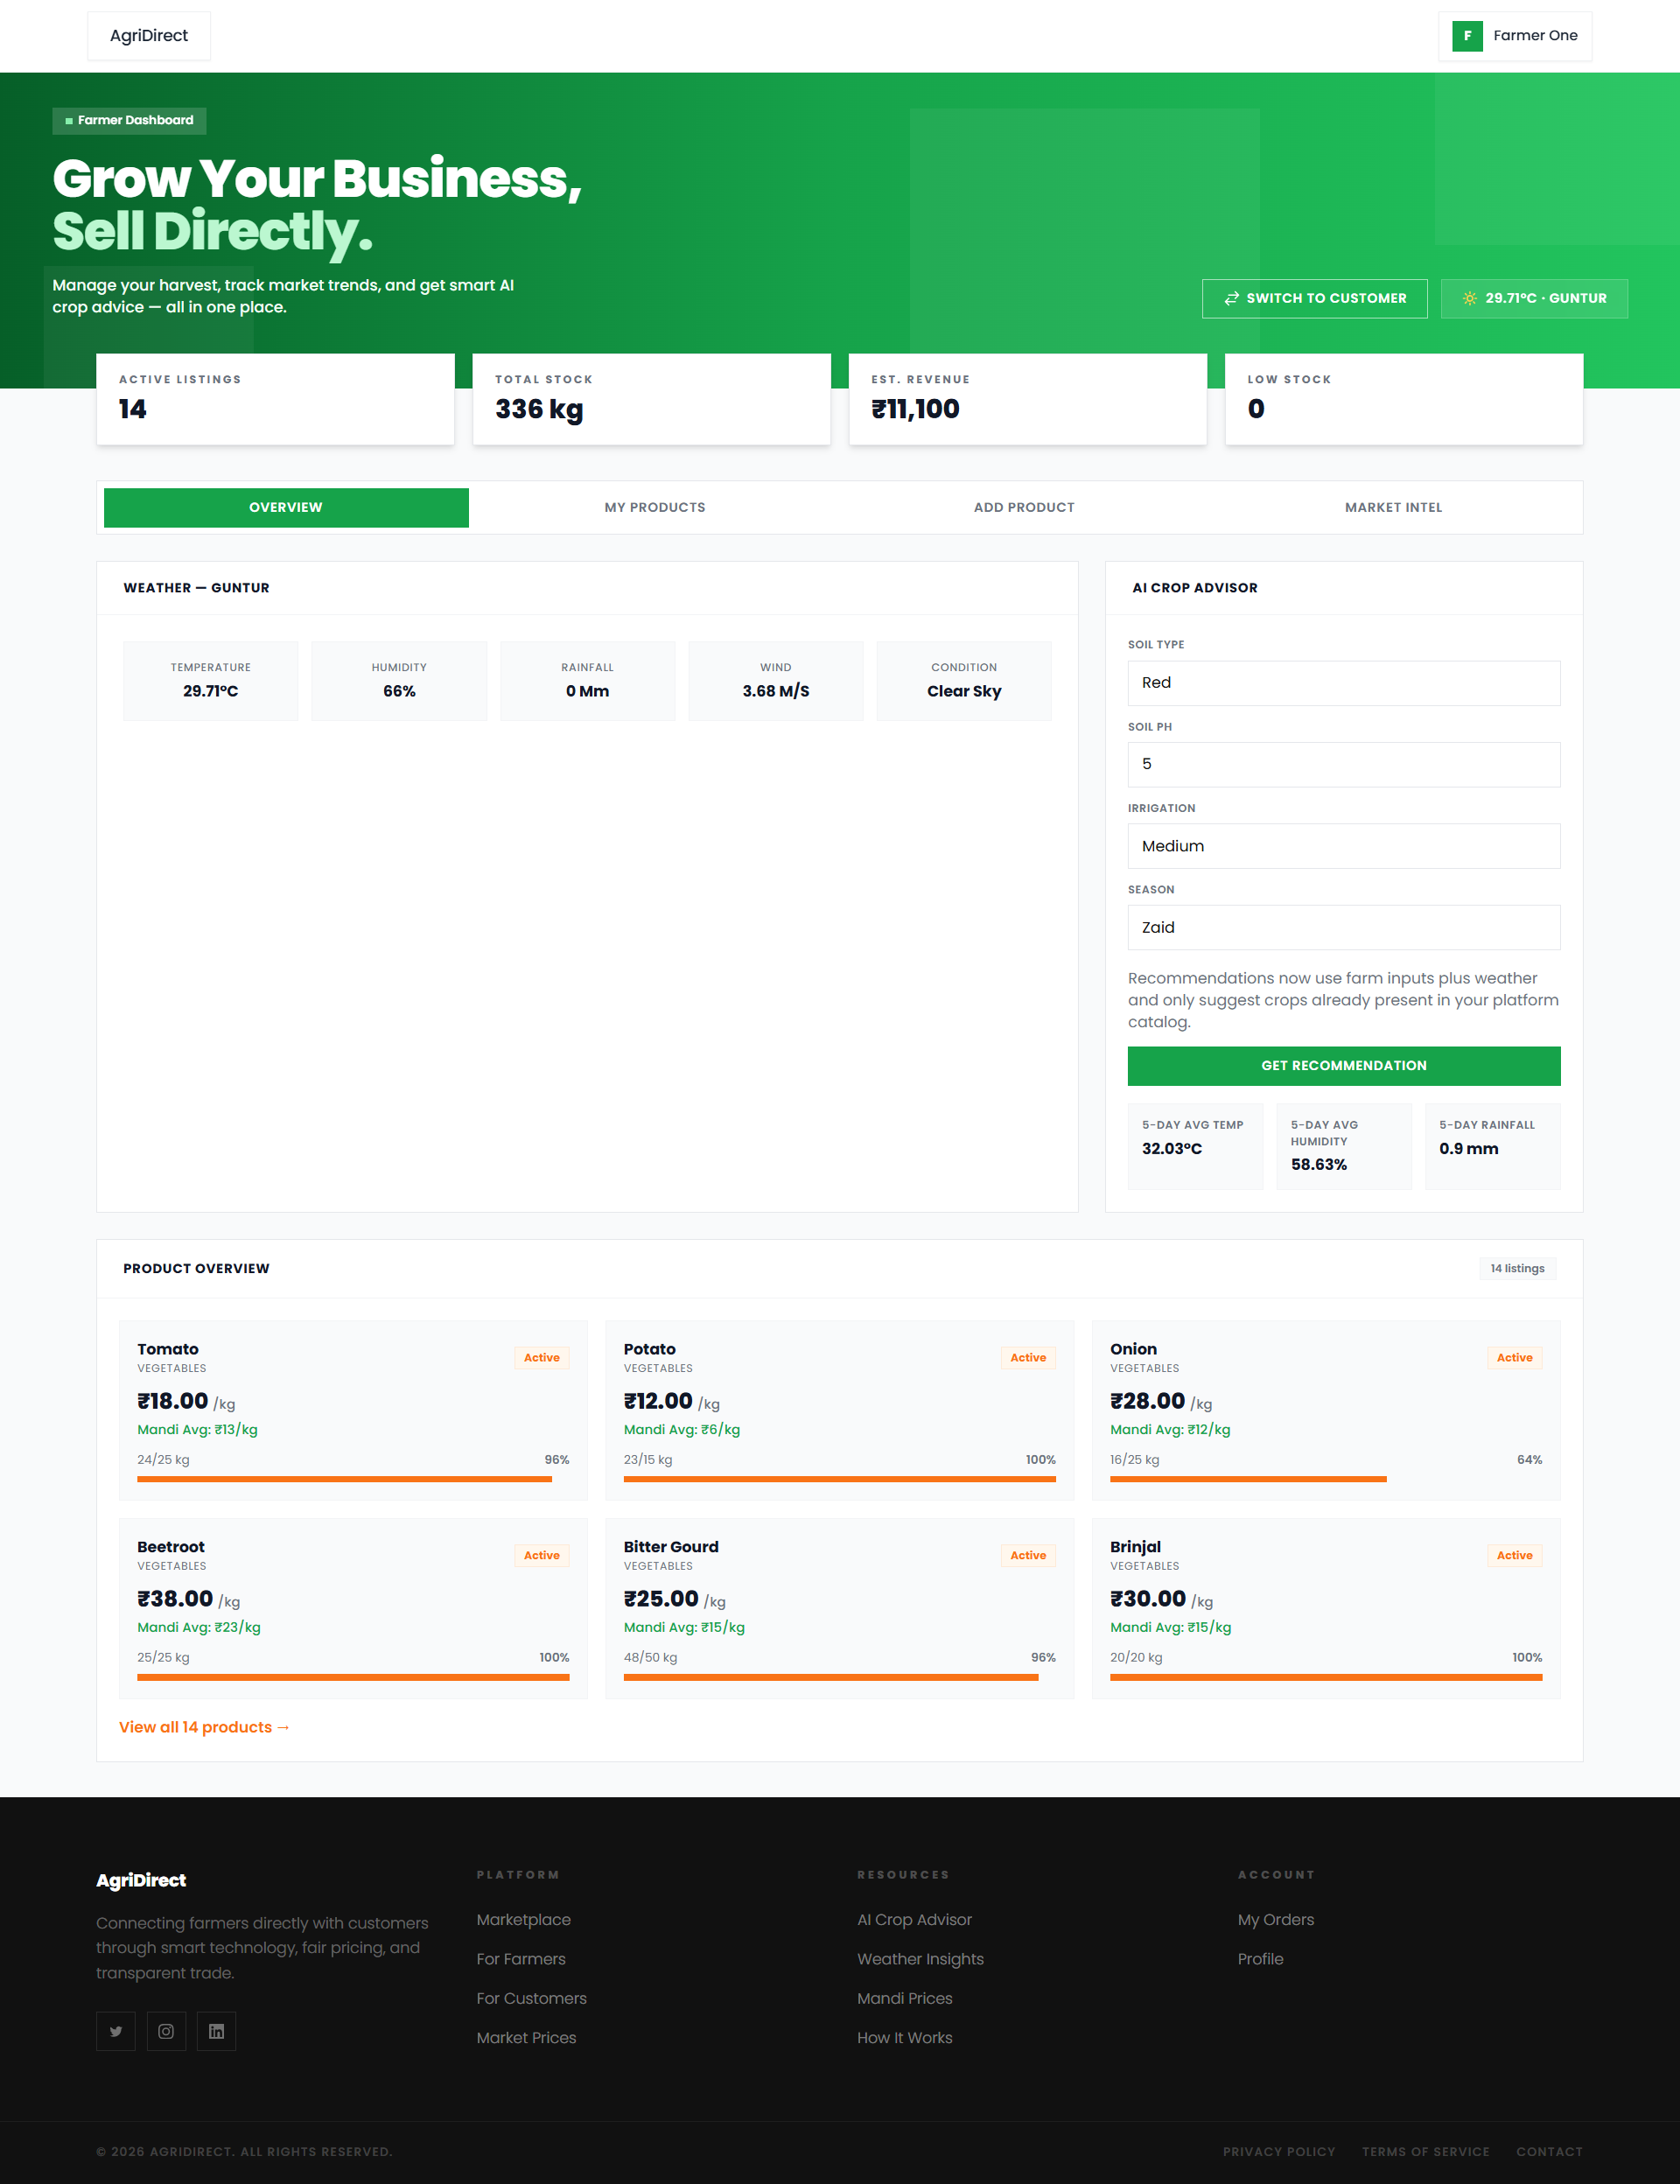
\includegraphics[width=0.48\textwidth]{farmer-dashboard.png}
\caption{Farmer dashboard of AgriDirect showing inventory overview, weather insights, AI crop advisory, and product summary.}
\label{fig:farmer-dashboard}
\end{figure}

\begin{figure}[htbp]
\centering
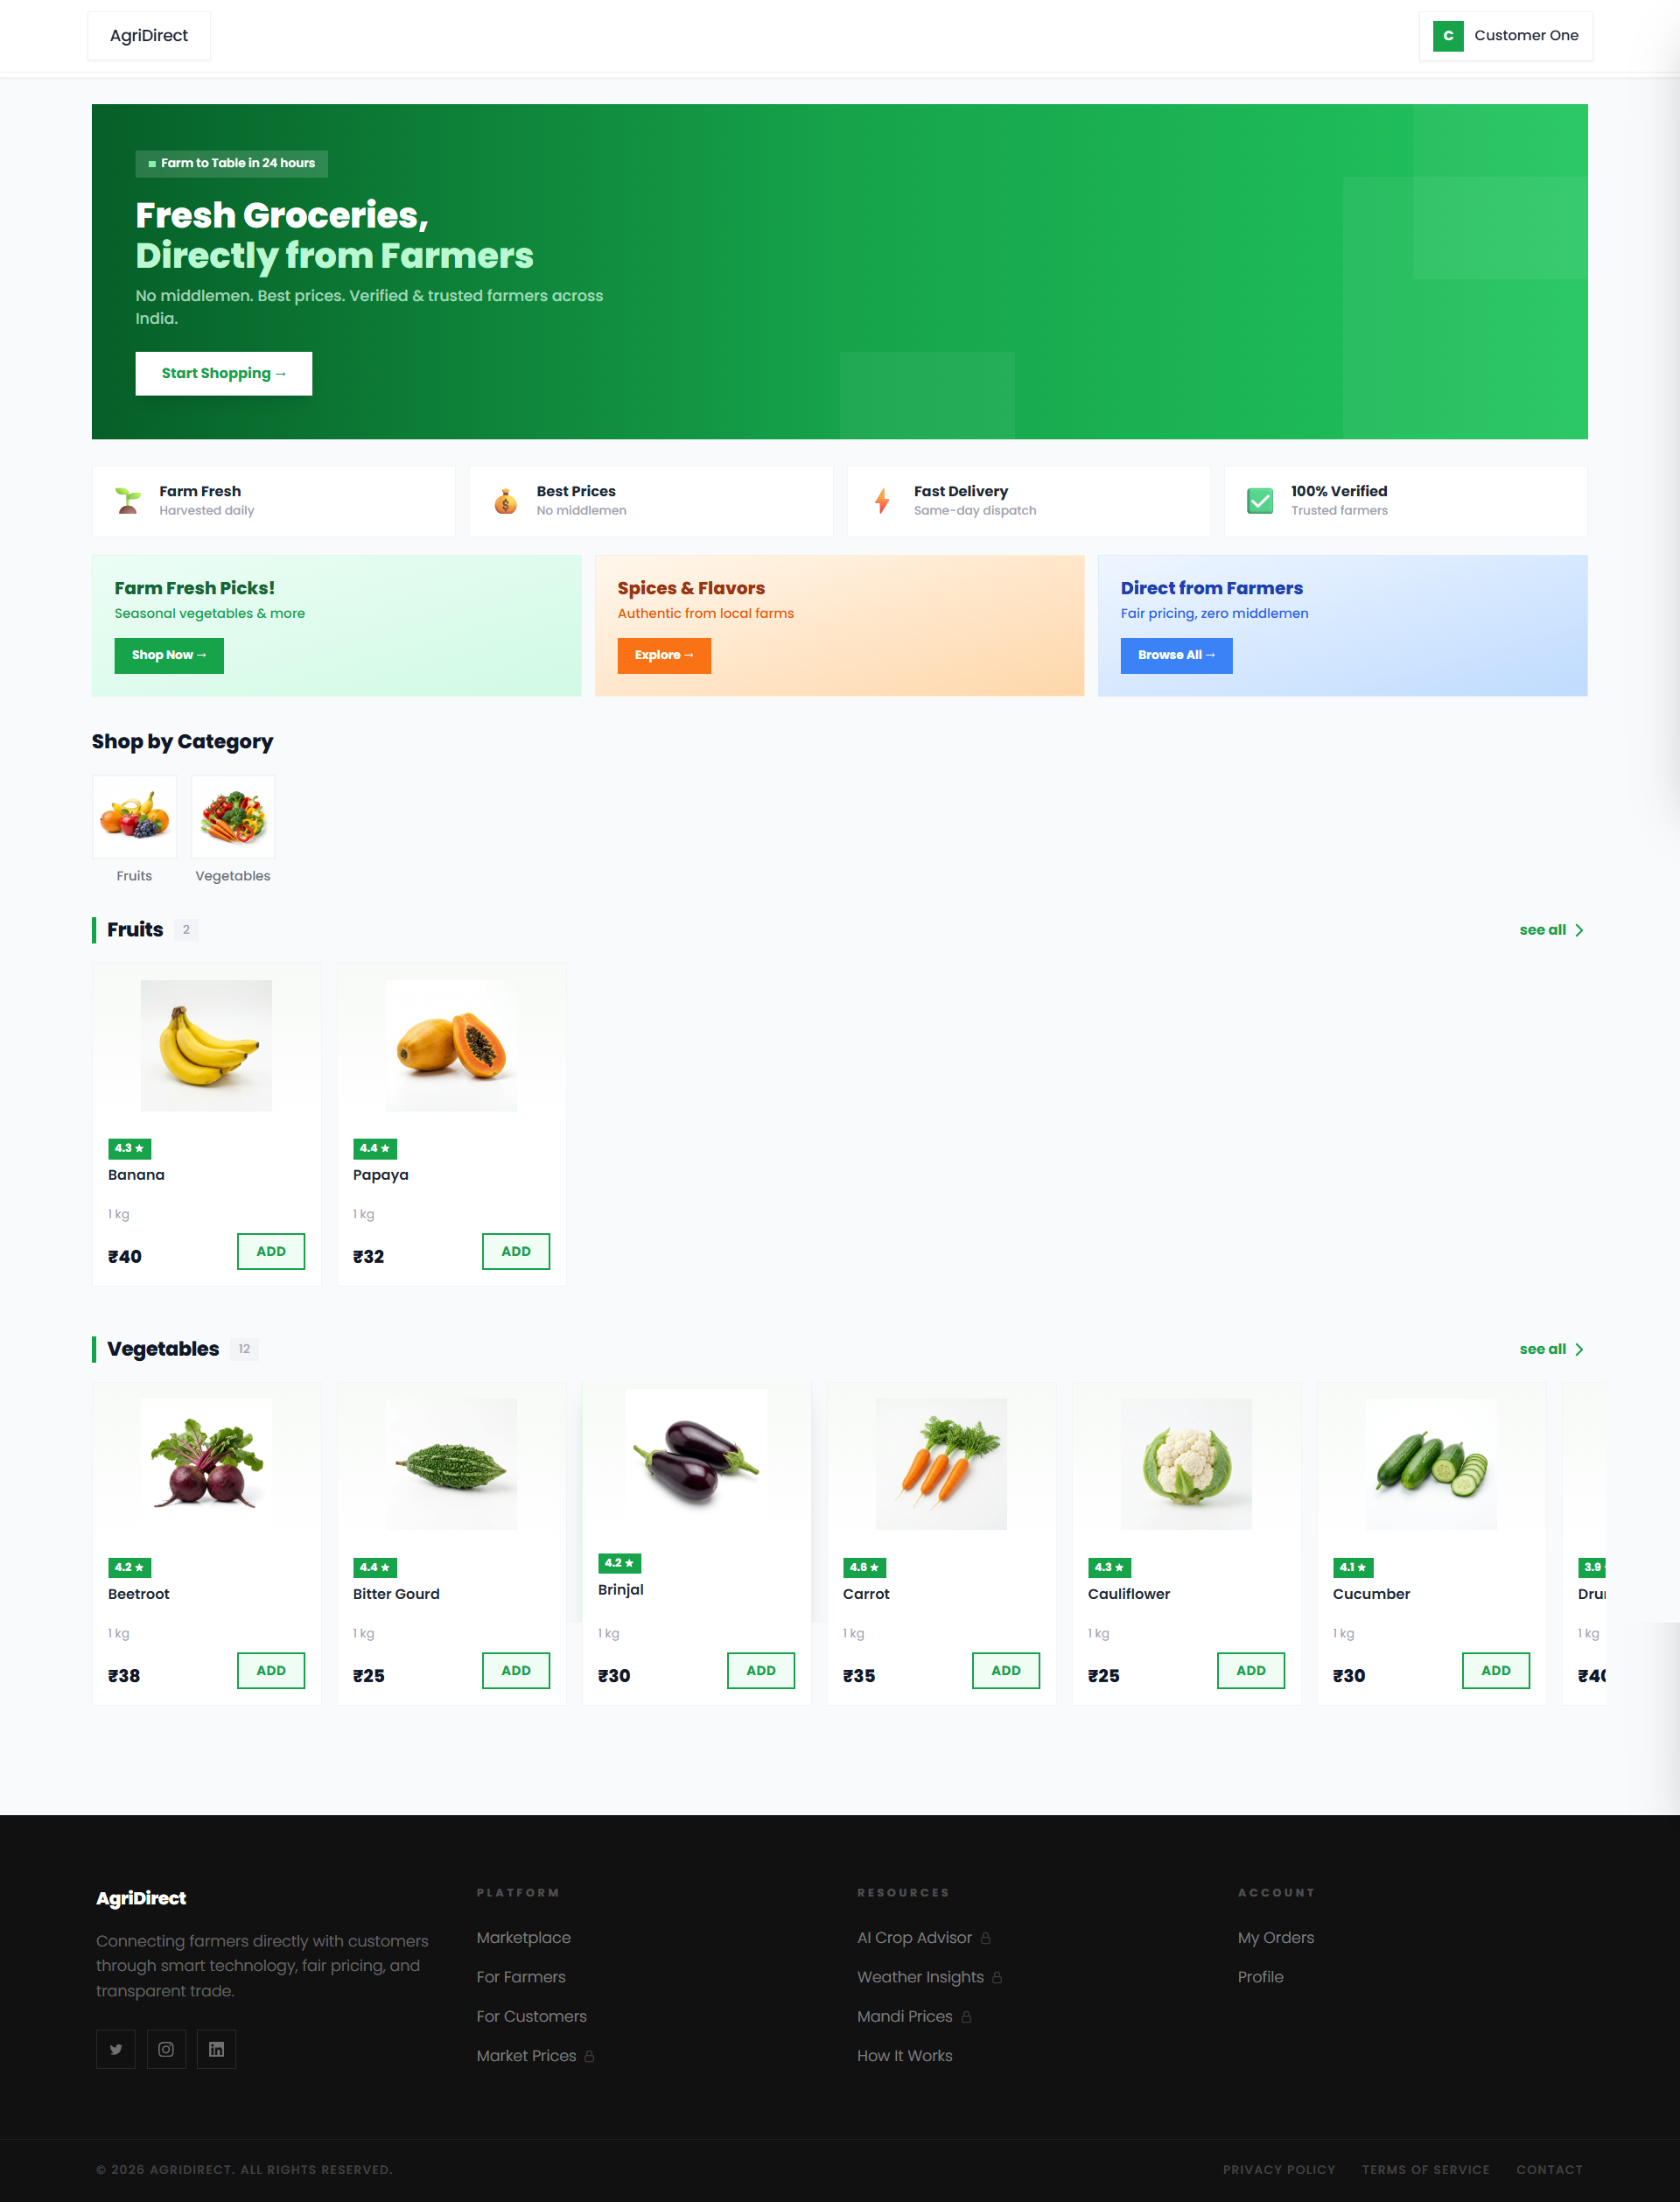
\includegraphics[width=0.48\textwidth]{customer-dashboard.png}
\caption{Customer marketplace interface showing grouped produce and direct discovery features.}
\label{fig:customer-marketplace}
\end{figure}

\section{Result and Discussion}
The implemented AgriDirect platform demonstrates that a marketplace can be strengthened by integrating agricultural intelligence instead of limiting itself to product listing and transaction handling. On the farmer side, the dashboard combines inventory status, weather summaries, live mandi prices, and crop recommendations in a single interface. On the customer side, the system provides grouped products, seller comparison, cart workflows, and location-aware sourcing.

The crop advisory workflow is a particularly important outcome of the system. Rather than using only a basic prediction model, the implemented service ranks crops through a hybrid process that combines farm suitability and market context. This makes the recommendations more practical for real decision making because the output reflects not only environmental conditions but also market opportunity.

Similarly, mandi analytics improve transparency by highlighting best markets, average modal prices, and price spread across records. This gives farmers additional signals for pricing and stocking decisions. Distance-aware seller discovery also adds value for customers who prefer nearby produce sources and potentially fresher inventory.

\subsection{Marketplace Output}
The customer-facing results of AgriDirect can be understood through grouped product displays, seller comparison panels, and cart-based order workflows. Instead of presenting every individual listing independently, the system aggregates similar products and then allows users to drill down into available sellers. This makes the interface cleaner and supports practical comparison among price, stock, and proximity.

On the farmer side, the inventory screen helps visualize active products, remaining quantity, calculated unit price, and corresponding mandi context. Such views support better stock awareness and can help farmers make informed listing and pricing updates.

\begin{figure}[htbp]
\centering
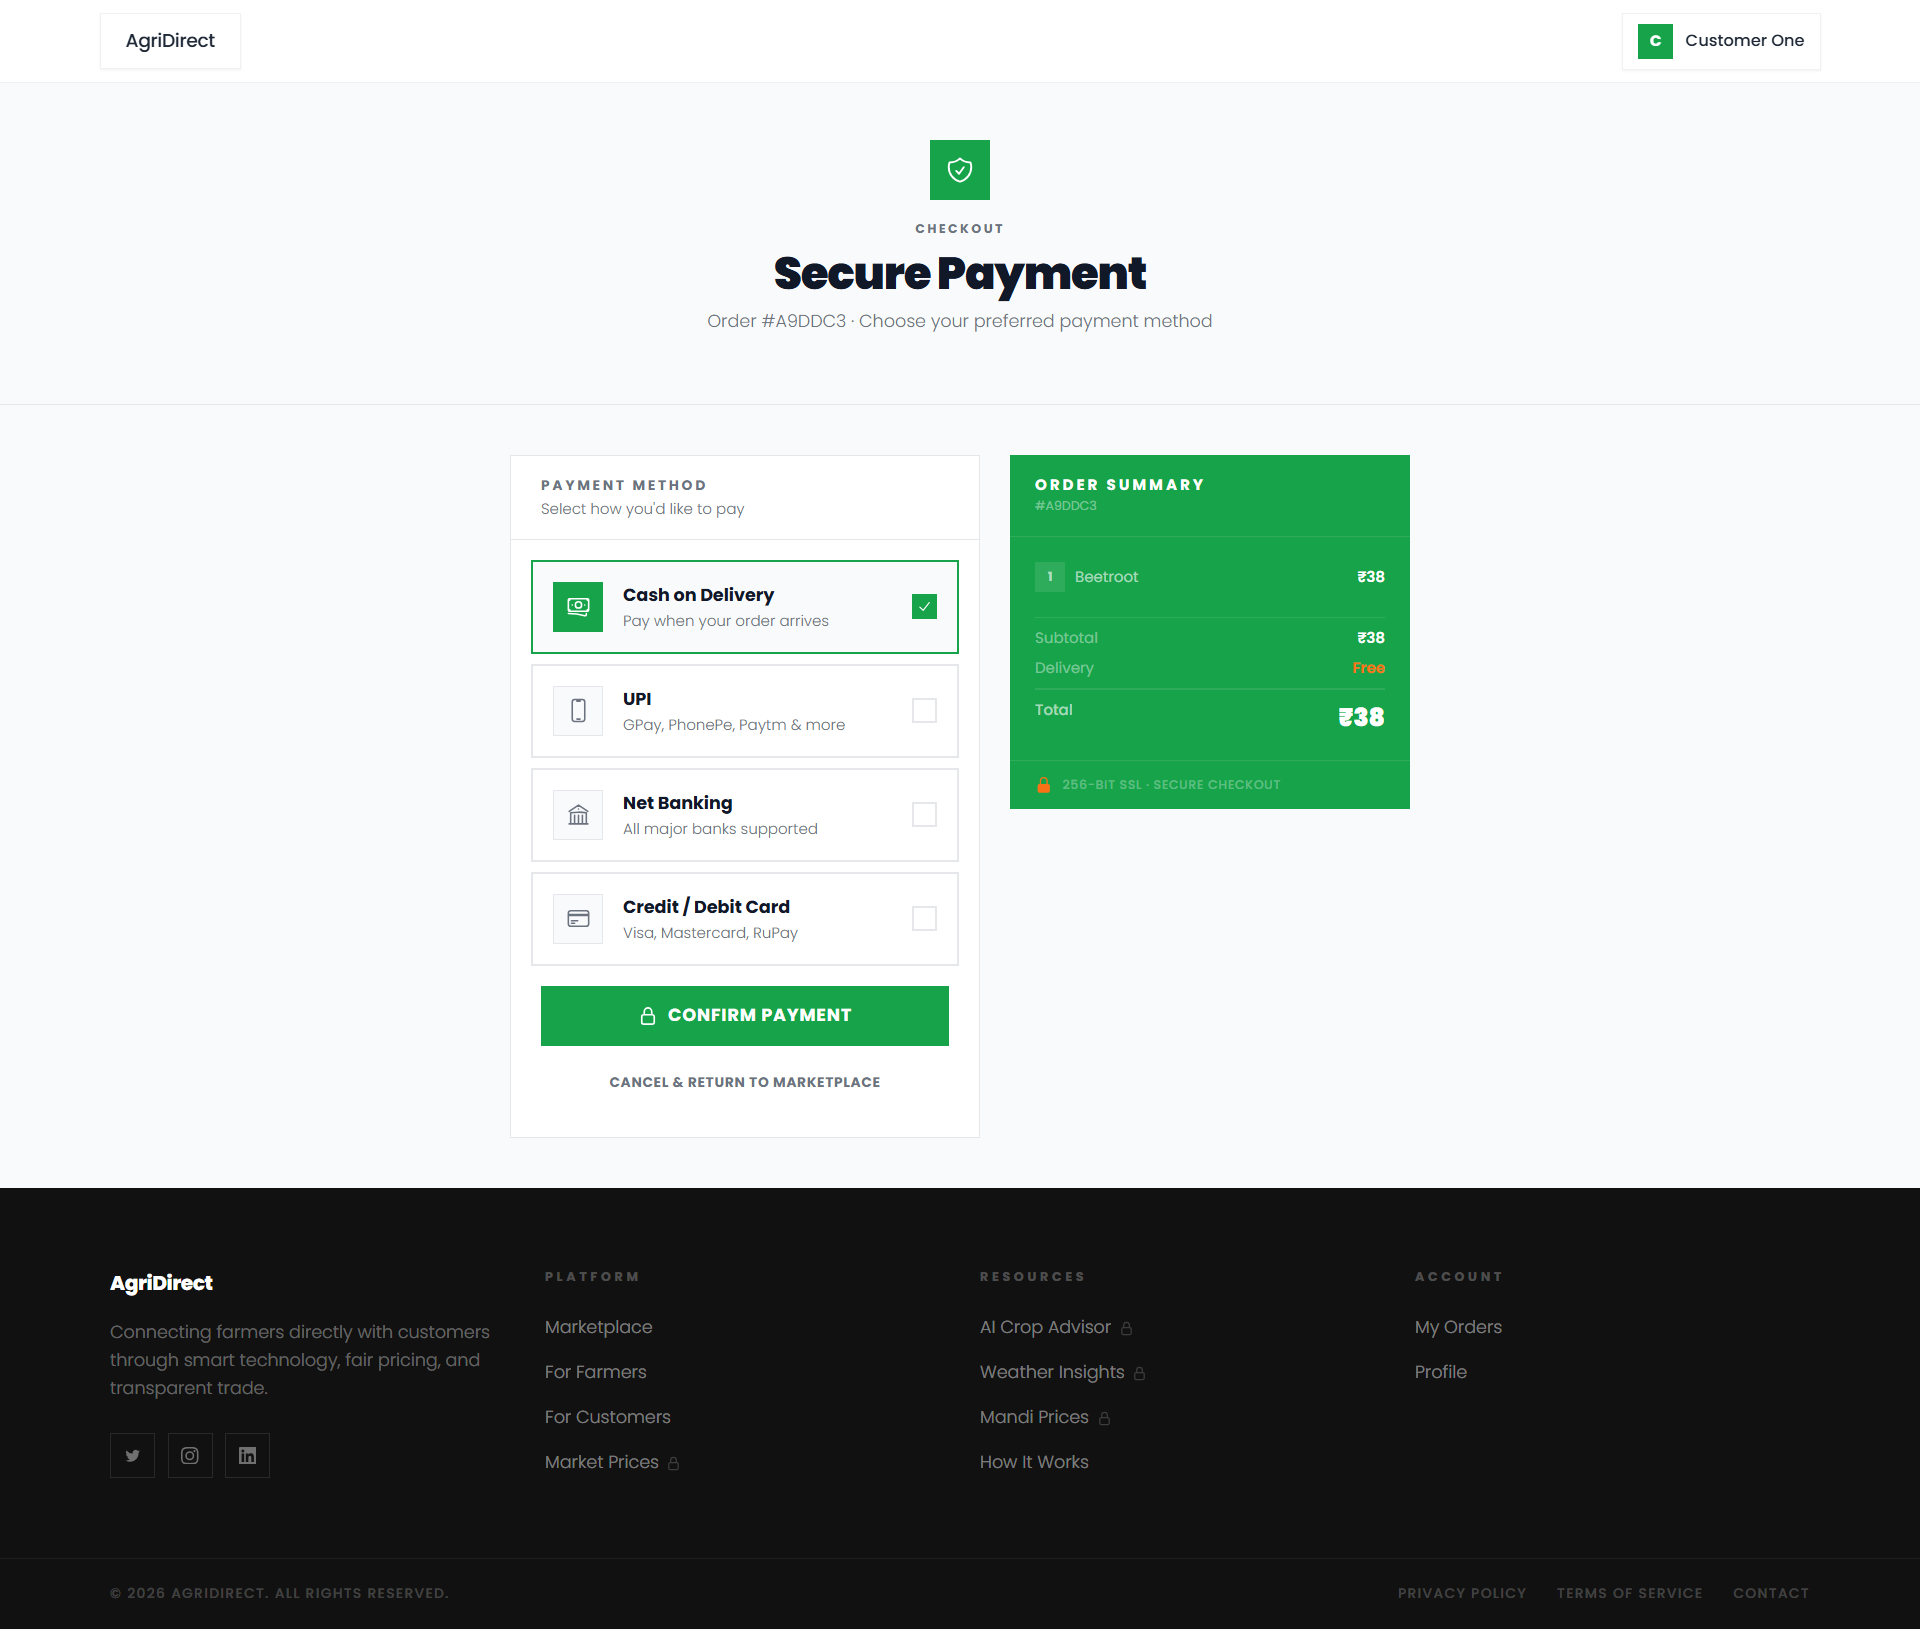
\includegraphics[width=0.48\textwidth]{cart.png}
\caption{Seller comparison and order workflow in AgriDirect.}
\label{fig:seller-cart}
\end{figure}

\subsection{Crop Advisory and Market Intelligence Output}
The advisory component produces ranked crop options instead of a single unqualified suggestion. Each recommendation is accompanied by confidence, suitability score, market bonus, and explanatory reasons. This improves interpretability and helps the farmer understand why one crop is favored over another. Since mandi data is used as a scoring factor, the system can distinguish between agronomically suitable crops and crops that are also supported by current market signals.

The mandi module also returns market-level summaries such as best market, lowest market, average price, and price spread. These outputs transform raw public data into directly usable signals for agricultural decision making.

\begin{figure}[htbp]
\centering
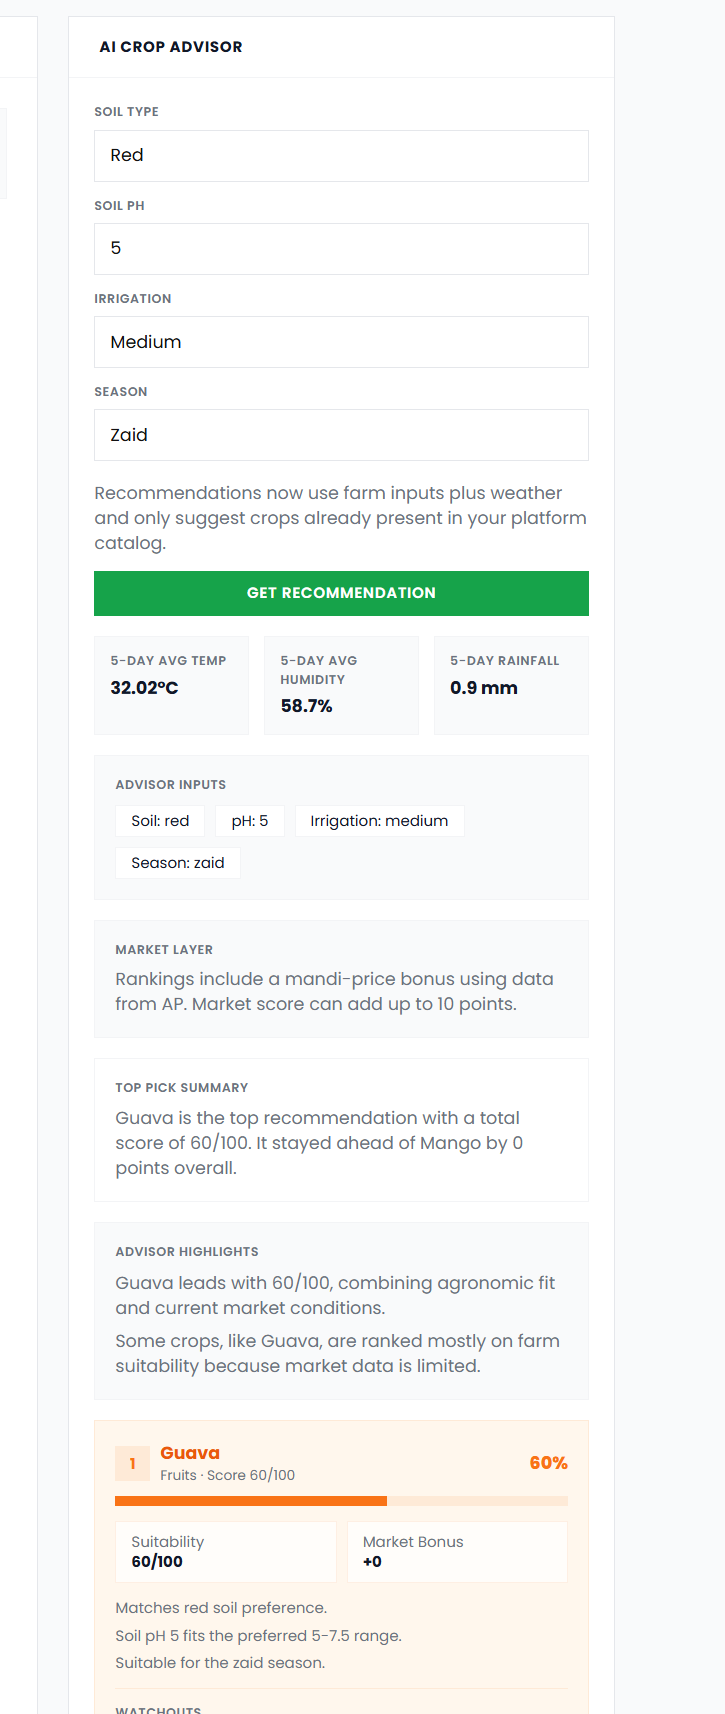
\includegraphics[width=0.48\textwidth]{crop-recommendation.png}
\caption{Weather-aware and market-aware crop recommendation output.}
\label{fig:crop-output}
\end{figure}

\begin{figure}[htbp]
\centering
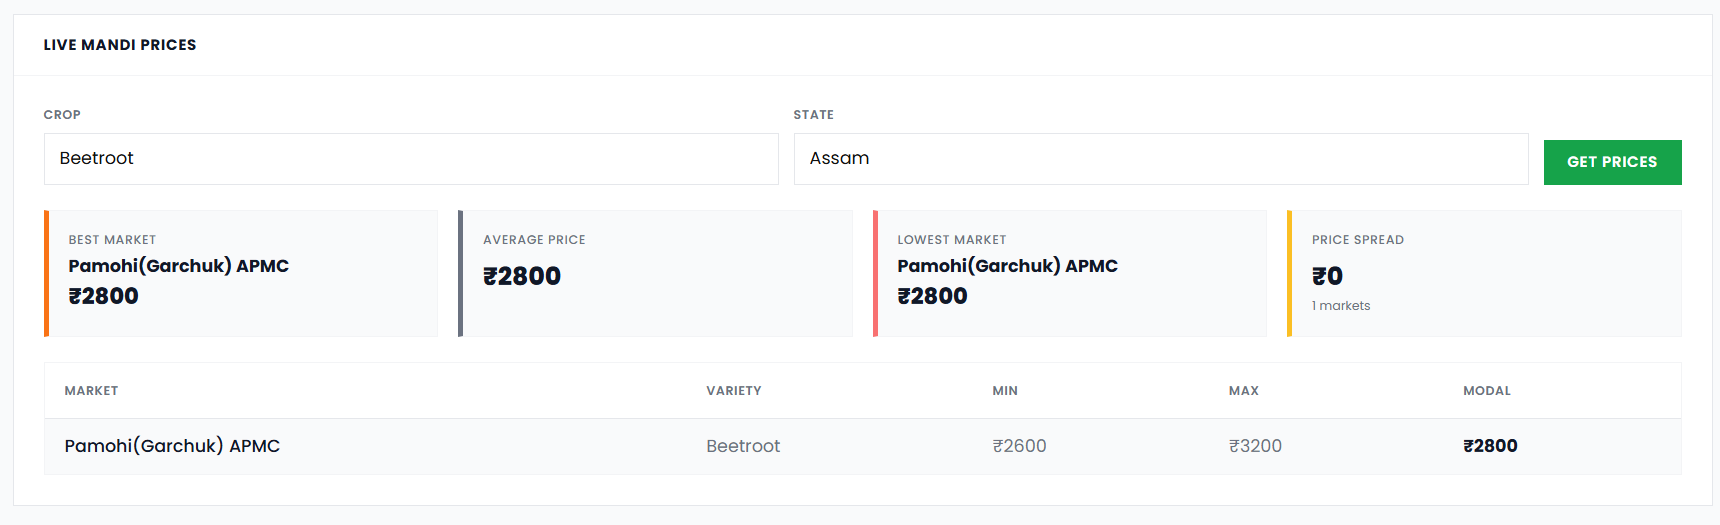
\includegraphics[width=0.48\textwidth]{mandi-prices.png}
\caption{Mandi price analytics interface in AgriDirect.}
\label{fig:mandi-output}
\end{figure}

\subsection{Model Evaluation View}
The reference paper includes evaluation-oriented visuals such as a confusion matrix and result graphics. To bring AgriDirect closer to that style, the crop recommendation module can be documented with machine learning evaluation outputs generated during model training. Since the model training script already computes accuracy, precision, recall, and F1-score, the paper can include those metrics together with a confusion matrix image exported from the training environment.

In the present draft, a placeholder is added for that evaluation figure. Once the actual confusion matrix is generated from the crop model, it can be inserted directly into the same location in Overleaf.

\begin{figure}[htbp]
\centering
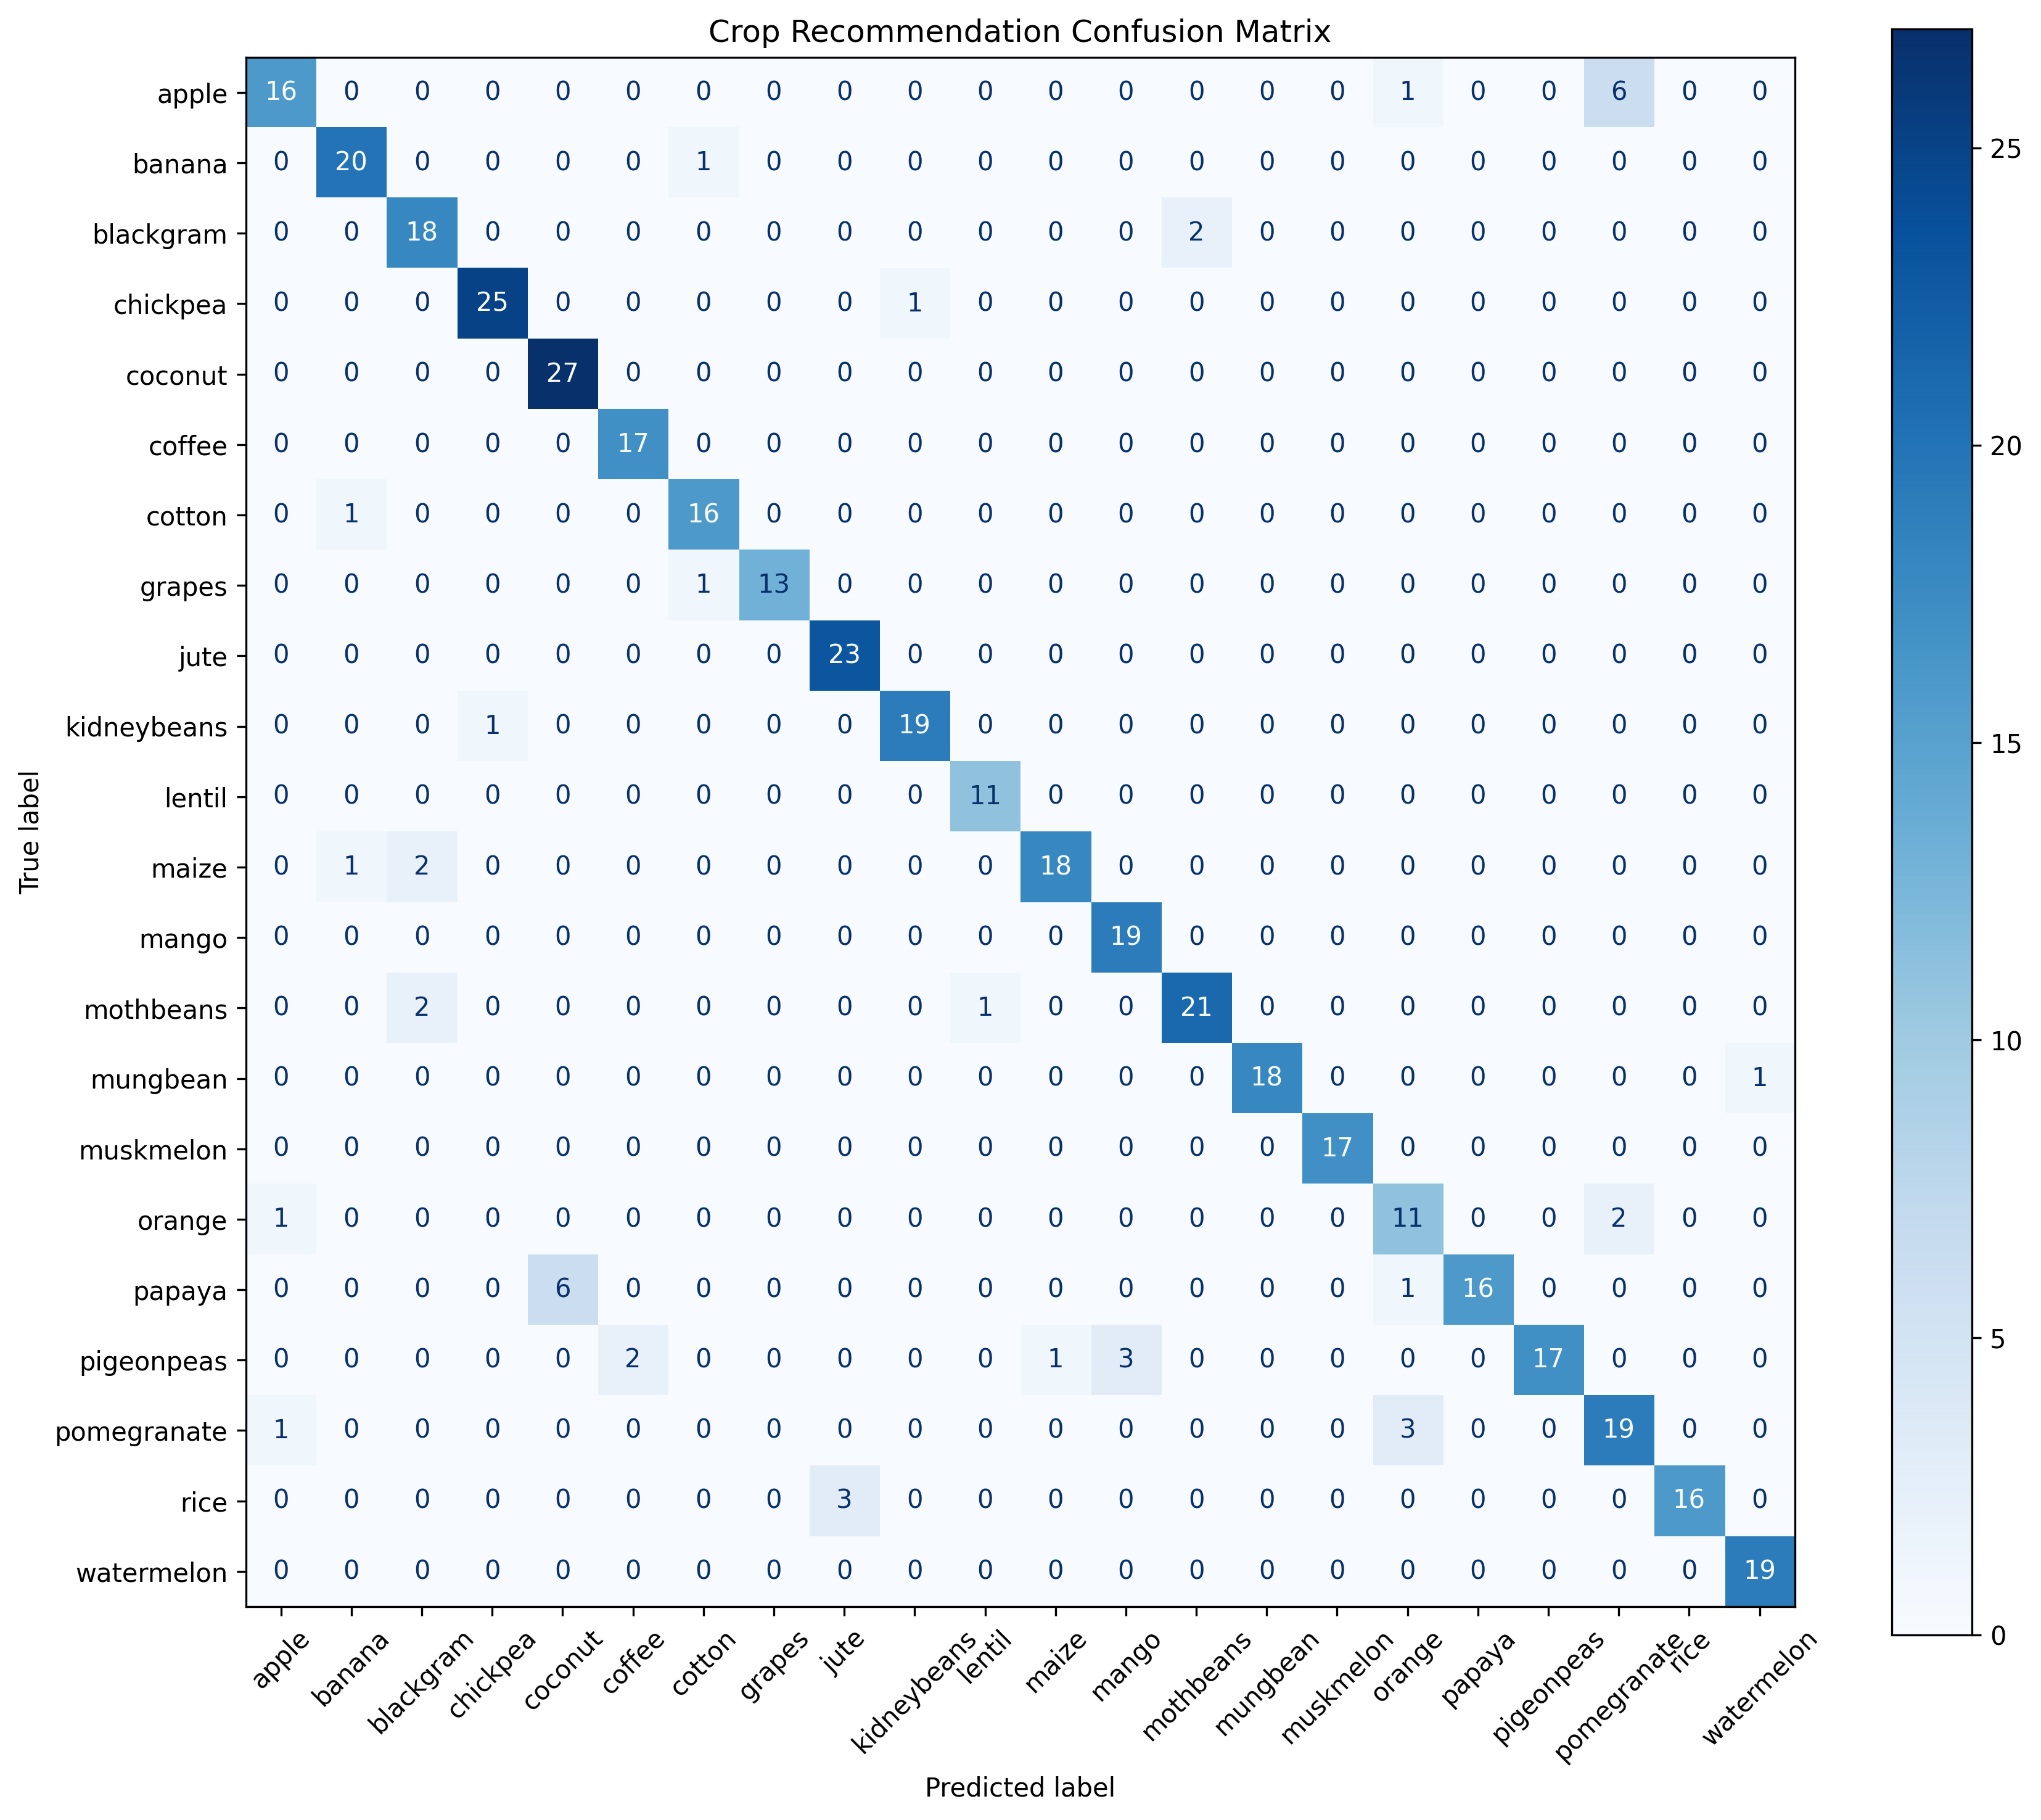
\includegraphics[width=0.48\textwidth]{confusion_matrix.png}
\caption{Confusion matrix or evaluation output for the crop recommendation model.}
\label{fig:confusion-matrix}
\end{figure}

\subsection{Discussion}
The major strength of AgriDirect lies in its integration. A standalone crop model may provide technically valid recommendations, but those outputs become more useful when they are tied to the actual marketplace inventory, mandi signals, and farmer workflow. Likewise, a marketplace becomes more valuable when it includes tools that support strategic farm planning instead of only order placement.

Another key observation is that the architecture supports incremental enhancement. The frontend can evolve with additional dashboards and visualizations, the backend can absorb new services such as logistics or notifications, and the machine learning layer can be retrained with richer data. This makes the system suitable not only as a student project but also as a foundation for a larger smart agriculture platform.

The proposed system offers several practical advantages:

\begin{enumerate}
\item direct digital linkage between farmers and customers;
\item improved price awareness through mandi analytics;
\item better crop planning through advisory support;
\item reduced friction in inventory and order management;
\item extensibility through service-oriented architecture;
\item location-aware seller comparison for customer convenience.
\end{enumerate}

Although AgriDirect demonstrates a useful integrated workflow, some limitations remain. The quality of recommendation output depends on the quality of user-supplied farm inputs and external weather or market feeds. The machine learning service currently operates on a limited feature set and can be improved further with richer soil, satellite, or seasonal datasets. In addition, platform-scale evaluation with real production usage is still needed to validate long-term impact.

Several enhancements are possible in future versions of AgriDirect:

\begin{enumerate}
\item multilingual interfaces for wider rural accessibility;
\item stronger recommendation models using larger agricultural datasets;
\item demand forecasting and harvest planning modules;
\item logistics and delivery tracking integration;
\item farmer ratings, trust scoring, and transaction analytics;
\item mobile application deployment for field use.
\end{enumerate}

\section{Conclusion}
AgriDirect presents an integrated agriculture platform that combines farm-to-customer e-commerce with intelligent advisory support. By connecting farmers, customers, market data, weather signals, and crop recommendation workflows, the system addresses both commercial and planning challenges in one environment. The project shows that practical digital agriculture platforms can go beyond simple listing and ordering features by embedding advisory intelligence directly into marketplace operations. As a result, AgriDirect provides a meaningful foundation for transparent trade, informed decision making, and scalable smart agriculture services.

\begin{thebibliography}{00}
\bibitem{b1} A. Gomathy and E. Boopathi Kumar, ``Farmer's Global Market Connecting Platform Using Supply Chain Management,'' \emph{World Journal of Advanced Research and Reviews}, vol. 26, no. 1, pp. 1700--1709, 2025.

\bibitem{b2} T. Reardon, M. F. Bellemare, and D. Zilberman, ``How E-Commerce and Digital Platforms Enhance Market Access for Farmers,'' \emph{Applied Economic Perspectives and Policy}, vol. 42, no. 1, pp. 3--19, 2020.

\bibitem{b3} A. Kamilaris, A. Fonts, and F. X. Prenafeta-Boldu, ``The Rise of Blockchain Technology in Agriculture and Food Supply Chains,'' \emph{Trends in Food Science and Technology}, vol. 91, pp. 640--652, 2019.

\bibitem{b4} H. Markelova, K. Meinzen-Dick, J. Hellin, and S. Dohrn, ``Collective Action for Smallholder Market Access,'' \emph{Food Policy}, vol. 34, no. 1, pp. 1--7, 2009.

\bibitem{b5} P. K. Shukla and R. K. Dubey, ``Smart Agriculture Market Using IoT and Artificial Intelligence,'' \emph{International Journal of Innovative Research in Computer and Communication Engineering}, vol. 10, no. 5, pp. 2310--2317, May 2022.

\bibitem{b6} M. R. Patel and A. D. Deshmukh, ``AI-Based Crop Prediction and Price Forecasting System for Farmers,'' \emph{International Journal of Advanced Research in Computer Science}, vol. 13, no. 4, pp. 45--51, 2022.

\bibitem{b7} S. Singh and A. Sharma, ``Farmer-to-Consumer Digital Marketplace: Bridging the Agricultural Gap,'' in \emph{IEEE International Conference on Smart Technologies for Smart Nation}, pp. 120--125, 2021.

\bibitem{b8} N. Kaur and S. Gupta, ``Enhancing Agricultural Trade Using Blockchain and Machine Learning,'' \emph{Journal of Emerging Technologies and Innovative Research}, vol. 8, no. 10, pp. 56--63, Oct. 2021.

\bibitem{b9} M. R. Bhardwaj \emph{et al.}, ``An Innovative Deep Learning Based Approach for Accurate Agricultural Crop Price Prediction,'' \emph{arXiv preprint arXiv:2304.09761}, 2023.

\bibitem{b10} L. Madaan \emph{et al.}, ``Price Forecasting and Anomaly Detection for Agricultural Commodities in India,'' in \emph{ACM COMPASS}, July 2019.

\bibitem{b11} A. Jain, S. Marvaniya, S. Godbole, and V. Munigala, ``Towards Context-Based Model Selection for Improved Crop Price Forecasting,'' in \emph{5th Joint International Conference on Data Science and Management of Data}, pp. 195--203, 2022.

\bibitem{b12} J. Fan \emph{et al.}, ``A GNN-RNN Approach for Harnessing Geospatial and Temporal Information: Application to Crop Yield Prediction,'' in \emph{Proceedings of the AAAI Conference on Artificial Intelligence}, vol. 36, pp. 11873--11881, 2022.

\bibitem{b13} A. Kumar and S. Sharma, ``Digital Transformation in Indian Agriculture,'' \emph{International Journal of Agricultural Science}, vol. 12, no. 3, pp. 45--52, 2020.

\bibitem{b14} Food and Agriculture Organization of the United Nations (FAO), ``E-Agriculture and Digital Innovation,'' 2020. Available: \url{https://www.fao.org/e-agriculture}.
\end{thebibliography}

\end{document}
